% Options for packages loaded elsewhere
\PassOptionsToPackage{unicode}{hyperref}
\PassOptionsToPackage{hyphens}{url}
%
\documentclass[
]{book}
\usepackage{amsmath,amssymb}
\usepackage{lmodern}
\usepackage{iftex}
\ifPDFTeX
  \usepackage[T1]{fontenc}
  \usepackage[utf8]{inputenc}
  \usepackage{textcomp} % provide euro and other symbols
\else % if luatex or xetex
  \usepackage{unicode-math}
  \defaultfontfeatures{Scale=MatchLowercase}
  \defaultfontfeatures[\rmfamily]{Ligatures=TeX,Scale=1}
\fi
% Use upquote if available, for straight quotes in verbatim environments
\IfFileExists{upquote.sty}{\usepackage{upquote}}{}
\IfFileExists{microtype.sty}{% use microtype if available
  \usepackage[]{microtype}
  \UseMicrotypeSet[protrusion]{basicmath} % disable protrusion for tt fonts
}{}
\makeatletter
\@ifundefined{KOMAClassName}{% if non-KOMA class
  \IfFileExists{parskip.sty}{%
    \usepackage{parskip}
  }{% else
    \setlength{\parindent}{0pt}
    \setlength{\parskip}{6pt plus 2pt minus 1pt}}
}{% if KOMA class
  \KOMAoptions{parskip=half}}
\makeatother
\usepackage{xcolor}
\usepackage{color}
\usepackage{fancyvrb}
\newcommand{\VerbBar}{|}
\newcommand{\VERB}{\Verb[commandchars=\\\{\}]}
\DefineVerbatimEnvironment{Highlighting}{Verbatim}{commandchars=\\\{\}}
% Add ',fontsize=\small' for more characters per line
\usepackage{framed}
\definecolor{shadecolor}{RGB}{248,248,248}
\newenvironment{Shaded}{\begin{snugshade}}{\end{snugshade}}
\newcommand{\AlertTok}[1]{\textcolor[rgb]{0.94,0.16,0.16}{#1}}
\newcommand{\AnnotationTok}[1]{\textcolor[rgb]{0.56,0.35,0.01}{\textbf{\textit{#1}}}}
\newcommand{\AttributeTok}[1]{\textcolor[rgb]{0.77,0.63,0.00}{#1}}
\newcommand{\BaseNTok}[1]{\textcolor[rgb]{0.00,0.00,0.81}{#1}}
\newcommand{\BuiltInTok}[1]{#1}
\newcommand{\CharTok}[1]{\textcolor[rgb]{0.31,0.60,0.02}{#1}}
\newcommand{\CommentTok}[1]{\textcolor[rgb]{0.56,0.35,0.01}{\textit{#1}}}
\newcommand{\CommentVarTok}[1]{\textcolor[rgb]{0.56,0.35,0.01}{\textbf{\textit{#1}}}}
\newcommand{\ConstantTok}[1]{\textcolor[rgb]{0.00,0.00,0.00}{#1}}
\newcommand{\ControlFlowTok}[1]{\textcolor[rgb]{0.13,0.29,0.53}{\textbf{#1}}}
\newcommand{\DataTypeTok}[1]{\textcolor[rgb]{0.13,0.29,0.53}{#1}}
\newcommand{\DecValTok}[1]{\textcolor[rgb]{0.00,0.00,0.81}{#1}}
\newcommand{\DocumentationTok}[1]{\textcolor[rgb]{0.56,0.35,0.01}{\textbf{\textit{#1}}}}
\newcommand{\ErrorTok}[1]{\textcolor[rgb]{0.64,0.00,0.00}{\textbf{#1}}}
\newcommand{\ExtensionTok}[1]{#1}
\newcommand{\FloatTok}[1]{\textcolor[rgb]{0.00,0.00,0.81}{#1}}
\newcommand{\FunctionTok}[1]{\textcolor[rgb]{0.00,0.00,0.00}{#1}}
\newcommand{\ImportTok}[1]{#1}
\newcommand{\InformationTok}[1]{\textcolor[rgb]{0.56,0.35,0.01}{\textbf{\textit{#1}}}}
\newcommand{\KeywordTok}[1]{\textcolor[rgb]{0.13,0.29,0.53}{\textbf{#1}}}
\newcommand{\NormalTok}[1]{#1}
\newcommand{\OperatorTok}[1]{\textcolor[rgb]{0.81,0.36,0.00}{\textbf{#1}}}
\newcommand{\OtherTok}[1]{\textcolor[rgb]{0.56,0.35,0.01}{#1}}
\newcommand{\PreprocessorTok}[1]{\textcolor[rgb]{0.56,0.35,0.01}{\textit{#1}}}
\newcommand{\RegionMarkerTok}[1]{#1}
\newcommand{\SpecialCharTok}[1]{\textcolor[rgb]{0.00,0.00,0.00}{#1}}
\newcommand{\SpecialStringTok}[1]{\textcolor[rgb]{0.31,0.60,0.02}{#1}}
\newcommand{\StringTok}[1]{\textcolor[rgb]{0.31,0.60,0.02}{#1}}
\newcommand{\VariableTok}[1]{\textcolor[rgb]{0.00,0.00,0.00}{#1}}
\newcommand{\VerbatimStringTok}[1]{\textcolor[rgb]{0.31,0.60,0.02}{#1}}
\newcommand{\WarningTok}[1]{\textcolor[rgb]{0.56,0.35,0.01}{\textbf{\textit{#1}}}}
\usepackage{longtable,booktabs,array}
\usepackage{calc} % for calculating minipage widths
% Correct order of tables after \paragraph or \subparagraph
\usepackage{etoolbox}
\makeatletter
\patchcmd\longtable{\par}{\if@noskipsec\mbox{}\fi\par}{}{}
\makeatother
% Allow footnotes in longtable head/foot
\IfFileExists{footnotehyper.sty}{\usepackage{footnotehyper}}{\usepackage{footnote}}
\makesavenoteenv{longtable}
\usepackage{graphicx}
\makeatletter
\def\maxwidth{\ifdim\Gin@nat@width>\linewidth\linewidth\else\Gin@nat@width\fi}
\def\maxheight{\ifdim\Gin@nat@height>\textheight\textheight\else\Gin@nat@height\fi}
\makeatother
% Scale images if necessary, so that they will not overflow the page
% margins by default, and it is still possible to overwrite the defaults
% using explicit options in \includegraphics[width, height, ...]{}
\setkeys{Gin}{width=\maxwidth,height=\maxheight,keepaspectratio}
% Set default figure placement to htbp
\makeatletter
\def\fps@figure{htbp}
\makeatother
\setlength{\emergencystretch}{3em} % prevent overfull lines
\providecommand{\tightlist}{%
  \setlength{\itemsep}{0pt}\setlength{\parskip}{0pt}}
\setcounter{secnumdepth}{5}
\usepackage{booktabs}
\ifLuaTeX
  \usepackage{selnolig}  % disable illegal ligatures
\fi
\usepackage[]{natbib}
\bibliographystyle{plainnat}
\IfFileExists{bookmark.sty}{\usepackage{bookmark}}{\usepackage{hyperref}}
\IfFileExists{xurl.sty}{\usepackage{xurl}}{} % add URL line breaks if available
\urlstyle{same} % disable monospaced font for URLs
\hypersetup{
  pdftitle={BIOSTATS},
  pdfauthor={Akira Terui},
  hidelinks,
  pdfcreator={LaTeX via pandoc}}

\title{BIOSTATS}
\author{Akira Terui}
\date{Last updated on 2022-09-16}

\begin{document}
\maketitle

{
\setcounter{tocdepth}{1}
\tableofcontents
}
\hypertarget{introduction}{%
\chapter*{Introduction}\label{introduction}}
\addcontentsline{toc}{chapter}{Introduction}

This textbook aims to introduce fundamental statistical techniques and their applications to biological data. A unique aspect of this book is the ``flipped-order'' introduction. Many statistics courses start with theory; yet, I found it difficult for those unfamiliar with statistics. I will start with a real example of the method, followed by the explanation for an underlying theory/concept. The author is an ecologist, so some methods in this book might not be popular in other fields.

\hypertarget{project-management}{%
\chapter{Project Management}\label{project-management}}

\hypertarget{r-project}{%
\section{R Project}\label{r-project}}

For this entire book, I will use \texttt{R\ Project} as a fundamental unit of work-space, in which all the relevant materials (e.g., R scripts \texttt{.R} and data files) are assembled together. There are many ways to organize your project, but I usually make a single \texttt{R\ Project} for a collection of scripts and data that will lead to a single publication (see example \href{https://github.com/aterui/public-proj_stream-diversity}{here}). To setup an \texttt{R\ Project} you will need \emph{R Studio} in addition to base \emph{R}. While \emph{R} is a stand-alone software, I strongly recommend to use it with \emph{R Studio}. \emph{R Studio} has many functions that help your data analysis. \emph{R} and \emph{R Studio} can be installed from the following websites:

\begin{itemize}
\tightlist
\item
  \href{https://www.r-project.org/}{R} (you can choose any CRAN mirror to download)
\item
  \href{https://rStudio.com/products/rStudio/download/}{R Studio}
\end{itemize}

Once you open \emph{R Studio}, you will see the following interface (Figure \ref{fig:ui}). There are three major panels in its first appearance -- \texttt{Console}, \texttt{Environment}, and \texttt{Files}. \texttt{Console} is the place where you write your codes and execute calculation/data manipulation/analysis. \texttt{Environment} lists items you saved as an object. \texttt{Files} list any files in a designated location in your computer.

\begin{figure}

{\centering 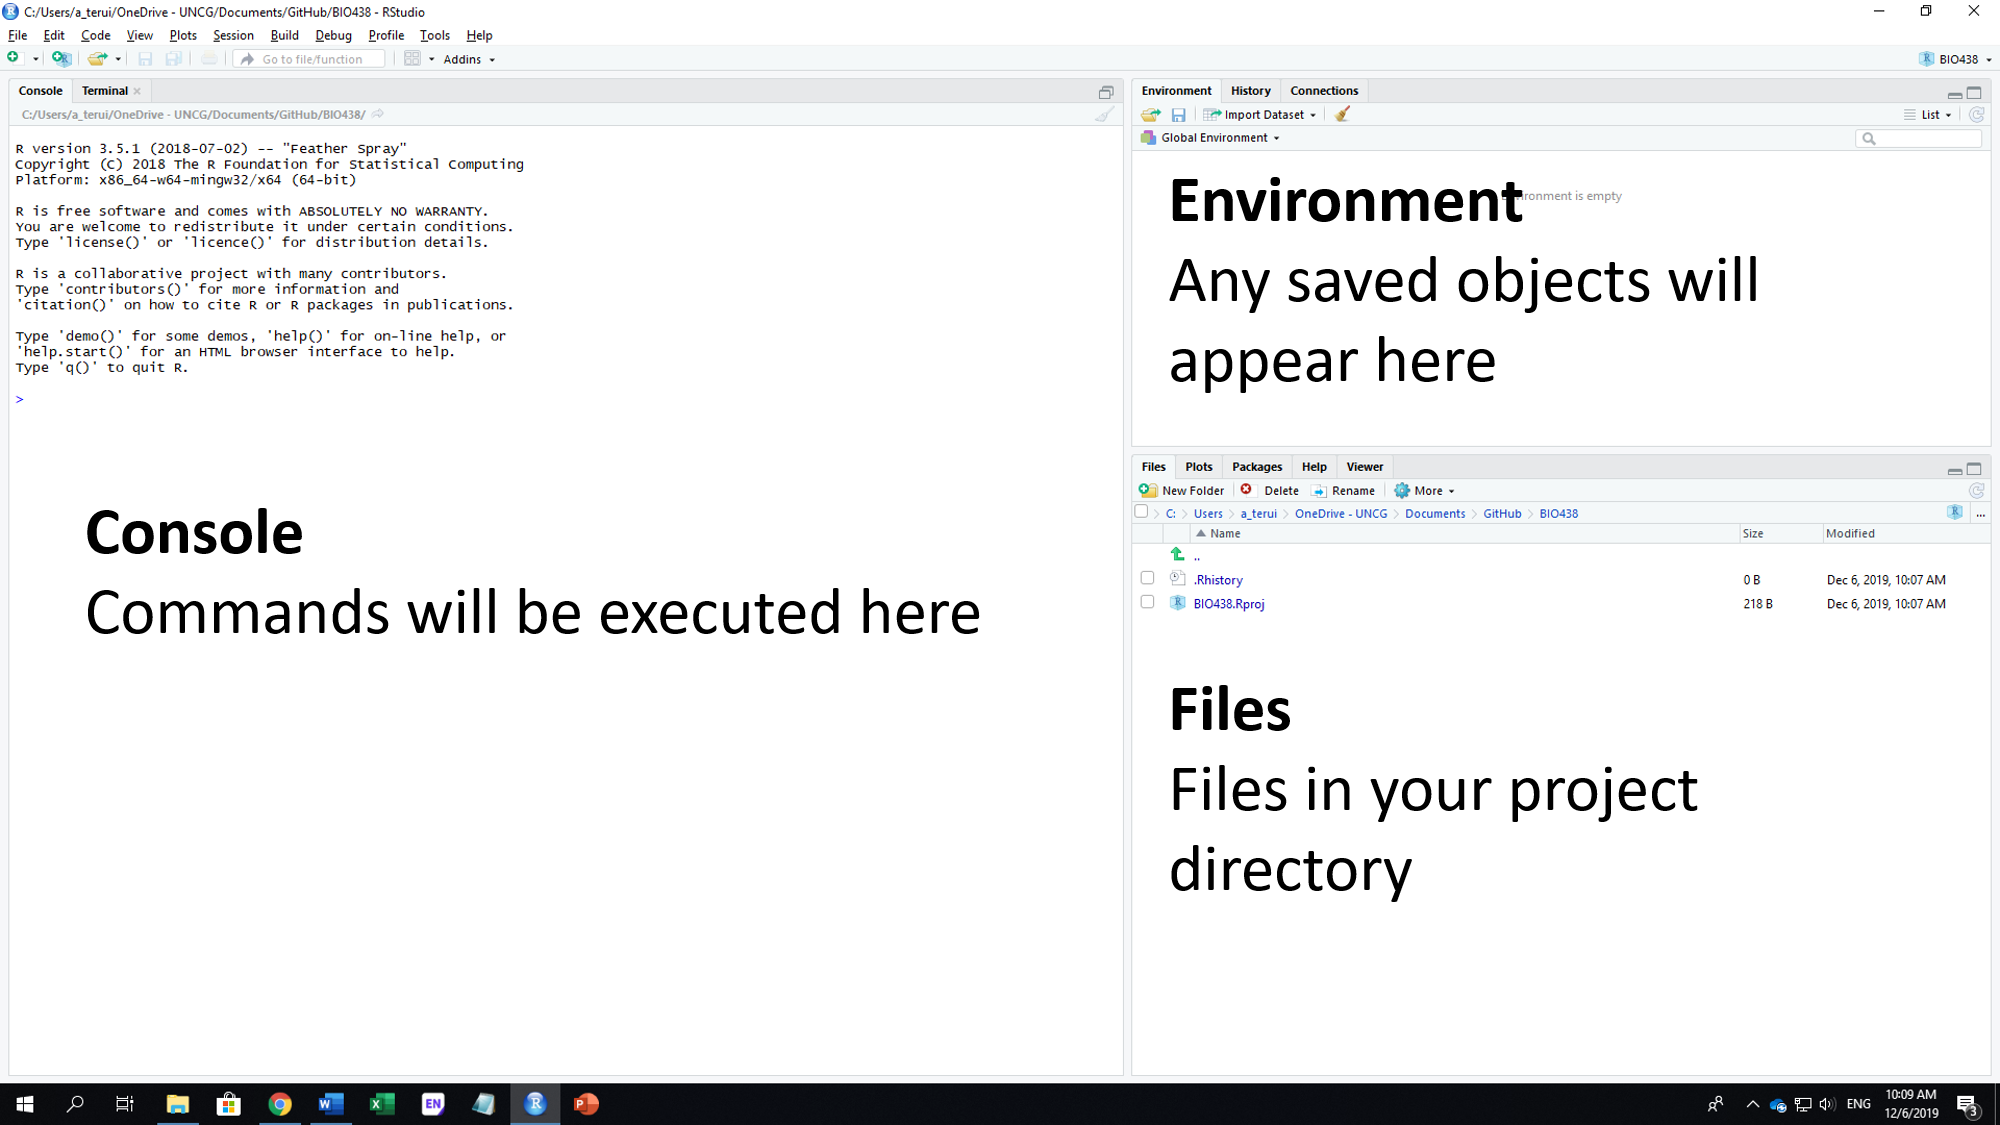
\includegraphics[width=9.47in]{image/r_image01} 

}

\caption{R Studio interface.}\label{fig:ui}
\end{figure}

Although you can work on your data as it appears, \textbf{it is actually a BAD idea}. As you work on your project, numerous materials will be generated. How do you manage files? If you randomly locate those materials within your computer, you will lose necessary items sooner or later. For this reason, I assemble all the relevant materials in a single \texttt{R\ Project}. You can create a new \texttt{R\ Project} with the following procedure.

\begin{enumerate}
\def\labelenumi{\alph{enumi}.}
\tightlist
\item
  Go to \texttt{File\ \textgreater{}\ New\ Project} on the top menu
\item
  Select \texttt{New\ Directory}
\item
  Select \texttt{New\ Project}
\end{enumerate}

A new window pops up and prompts you to name a directory with a location in your computer. Click \texttt{Browse} to select a location for the directory.

\textbf{IMPORTANT:} When you locate your project directories in your computer, I would strongly recommend to create a designated space. For example, in my computer, I have a folder named /\texttt{r\_project} in which all the \texttt{R\ Project} directories are located.

\hypertarget{internal-structure}{%
\section{Internal Structure}\label{internal-structure}}

The internal structure of an \texttt{R\ Project} is extremely important to navigate yourself (others once it's published). \texttt{R\ Project} will be composed of multiple types of files, typically \texttt{.R}, \texttt{.csv}, \texttt{.rds}, \texttt{.Rmd} among others. Unless those files are arranged in an organized manner, it is VERY LIKELY to make severe errors in coding. So I take this seriously. Table \ref{tab:str} is my suggested subdirectory structure.

\begin{longtable}[]{@{}
  >{\raggedright\arraybackslash}p{(\columnwidth - 2\tabcolsep) * \real{0.2639}}
  >{\raggedright\arraybackslash}p{(\columnwidth - 2\tabcolsep) * \real{0.7361}}@{}}
\caption{\label{tab:str} Suggested internal structure of \texttt{R\ Project}}\tabularnewline
\toprule()
\begin{minipage}[b]{\linewidth}\raggedright
Name
\end{minipage} & \begin{minipage}[b]{\linewidth}\raggedright
Content
\end{minipage} \\
\midrule()
\endfirsthead
\toprule()
\begin{minipage}[b]{\linewidth}\raggedright
Name
\end{minipage} & \begin{minipage}[b]{\linewidth}\raggedright
Content
\end{minipage} \\
\midrule()
\endhead
\texttt{README.md} & Markdown file explaining contents in the \texttt{R\ Project}. Can be derived from \texttt{README.Rmd}. \\
\texttt{/code} & Sub-directory for R scripts (\texttt{.R}). \\
\texttt{/data\_raw} & Sub-directory for raw data before data manipulation (\texttt{.csv} or other formats). Files in this sub-directory MUST NOT be modified unless there are changes to raw data entries. \\
\texttt{/data\_format} & Sub-directory for formatted data (\texttt{.csv}, \texttt{.rds}, or other formats). \\
\texttt{/output} & Sub-directory for result outputs (\texttt{.csv}, \texttt{.rds}, or other formats). This may include statistical estimates from linear regression models etc. \\
\texttt{/rmd} & (Optional) Sub-directory for Rmarkdown files (\texttt{.Rmd}). Rmarkdown allows seamless integration of R scripts and text. \\
\bottomrule()
\end{longtable}

\hypertarget{file-name}{%
\section{File Name}\label{file-name}}

It is also critical to have \textbf{consistent naming rules} for your files. As you make progress on your project, the number of files in each sub-directory will increase, perhaps exponentially. You will find it difficult navigating yourself unless you have clear naming rules for files (and even worse for others). Here are some recommendations:

\begin{itemize}
\tightlist
\item
  \textbf{NO SPACE.} Use underscore.

  \begin{itemize}
  \tightlist
  \item
    Do: \texttt{script\_week1.R}
  \item
    Don't: \texttt{script\ week1.R}
  \end{itemize}
\item
  \textbf{NO UPPERCASE.} Use lowercase for file names.

  \begin{itemize}
  \tightlist
  \item
    Do: \texttt{script\_week1.R}
  \item
    Don't: \texttt{Script\_week1.R}
  \end{itemize}
\item
  \textbf{BE CONSISTENT.} Apply consistent naming rules within a project.

  \begin{itemize}
  \tightlist
  \item
    Do: R scripts for figures always start with a common prefix, e.g., \texttt{figure\_XXX.R} \texttt{figure\_YYY.R}(\texttt{XXX} and \texttt{YYY} specifies further details).
  \item
    Don't: R scripts for figures start with random text, e.g., \texttt{XXX\_fig.R} , \texttt{Figure\_Y2.R} , \texttt{plotB.R}.
  \end{itemize}
\end{itemize}

\hypertarget{robust-coding}{%
\section{Robust coding}\label{robust-coding}}

While this is not mandatory, I strongly recommend to use \emph{R Studio} with \emph{Git} \& \emph{GitHub} (see Chapter \ref{appendix} Appendix for guidance). Coding is innately error-prone\footnote{well WAY BETTER than manual data manipulation!}; every programmers, even bright ones, make mistakes - no exception. However, the critical difference between beginner and advanced programmers is whether they develop robust coding rules with a self-error-detection system. \emph{Git} is the key to this. I will touch on this occasionally throughout this book.

\hypertarget{appendix}{%
\chapter{Appendix}\label{appendix}}

\hypertarget{git-github}{%
\section{\texorpdfstring{\emph{Git} \& \emph{GitHub}}{Git \& GitHub}}\label{git-github}}

In this section, I will cover how to integrate \emph{Git} and \emph{GitHub} into \emph{R Studio}. \emph{R Studio} is excellent as is, but it becomes even better when combined with \emph{Git} and \emph{GitHub}. \emph{Git} is a free and open source distributed version control system. \textbf{\emph{Git}} \textbf{tracks changes in your codes codes while you work on your project so you are aware of any changes you made to your script (and other) files}. Tracking changes is extremely important to avoid unintended errors in your codes. This feature also helps avoid creating redundant files. While \emph{Git} is a local system, it has an online counterpart called \emph{GitHub}.

To make this system work, you'll need to go through some processes. The first step is to install \emph{Git} onto your computer:

\begin{itemize}
\item
  \textbf{Windows}: Install \emph{Git} from \href{https://gitforwindows.org/}{here}. You will be asked about ``Adjusting your PATH environment''. Choose ``\emph{Git} from the command line and also from 3rd-party software'' if it is not selected.
\item
  \textbf{Mac}: Follow the instruction \href{https://happygitwithr.com/install-git.html}{here}.
\end{itemize}

Then open R Studio and do \texttt{Create\ Project} \textgreater{} \texttt{New\ Directory} \textgreater{} \texttt{New\ Project}. If you see a check box \texttt{Create\ a\ git\ repository}, check and create a new project (Figure \ref{fig:gitcheck}). You will see a \emph{Git} pane on the upper right panel.

\begin{figure}

{\centering 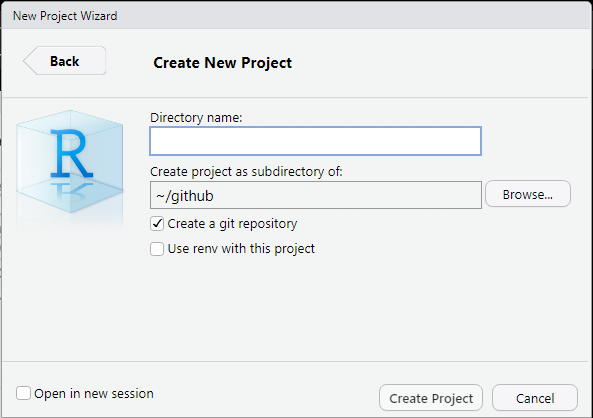
\includegraphics[width=8.24in]{image/git_image01} 

}

\caption{After installing Git, you should see `Create a git repository`.}\label{fig:gitcheck}
\end{figure}

If you can't find the above, do the following: \texttt{Tools} in the menu bar \textgreater{} \texttt{Terminal} \textgreater{} \texttt{New\ Terminal}, and type \texttt{where\ git} in the terminal. This will tell you where git executable is located in your computer. Then, go to \texttt{Tools} in the menu bar \textgreater{} \texttt{Global\ Options} \textgreater{} \texttt{Git/SVN}. You will see \emph{Git executable} in the box, where you can specify the location of git executable.

Next, go to \href{https://github.com/}{\emph{GitHub}} and create your account (free!). But, give some thoughts on your user name. My advice is the following. First, \textbf{use lowercase only.} Second, \textbf{include your name} to make it easy to find you on \emph{GitHub}.

\emph{R Studio} works seamlessly with \emph{Git} or \emph{GitHub}, but it is helpful to use a \emph{Git client} as it provides visual aids. There are choices for a \emph{Git client} (see options \href{https://happygitwithr.com/git-client.html}{here}) but I will use \emph{GitHub Desktop} (available \href{https://desktop.github.com/}{here}) for our exercise. Install GitHub Desktop onto you computer.

\hypertarget{commit-push}{%
\section{Commit \& Push}\label{commit-push}}

\hypertarget{register-your-git-repo}{%
\subsection{Register Your Git repo}\label{register-your-git-repo}}

Open the \texttt{R\ Project} you've just created as a git repository. Let's make a sample \texttt{.R} file (\texttt{Ctr\ +\ Shift\ +\ N}) and save it (name as \texttt{sample.R}). For example:

\begin{Shaded}
\begin{Highlighting}[]
\DocumentationTok{\#\# produce 100 random numbers that follows a normal distribution}
\NormalTok{x }\OtherTok{\textless{}{-}} \FunctionTok{rnorm}\NormalTok{(}\DecValTok{100}\NormalTok{, }\AttributeTok{mean =} \DecValTok{0}\NormalTok{, }\AttributeTok{sd =} \DecValTok{1}\NormalTok{)}

\DocumentationTok{\#\# estimate mean}
\FunctionTok{mean}\NormalTok{(x)}

\DocumentationTok{\#\# estimate SD}
\FunctionTok{sd}\NormalTok{(x)}
\end{Highlighting}
\end{Shaded}

Open GitHub Desktop App. You will see the following GUI (Figure \ref{fig:gitdesktop1}):

\begin{figure}

{\centering 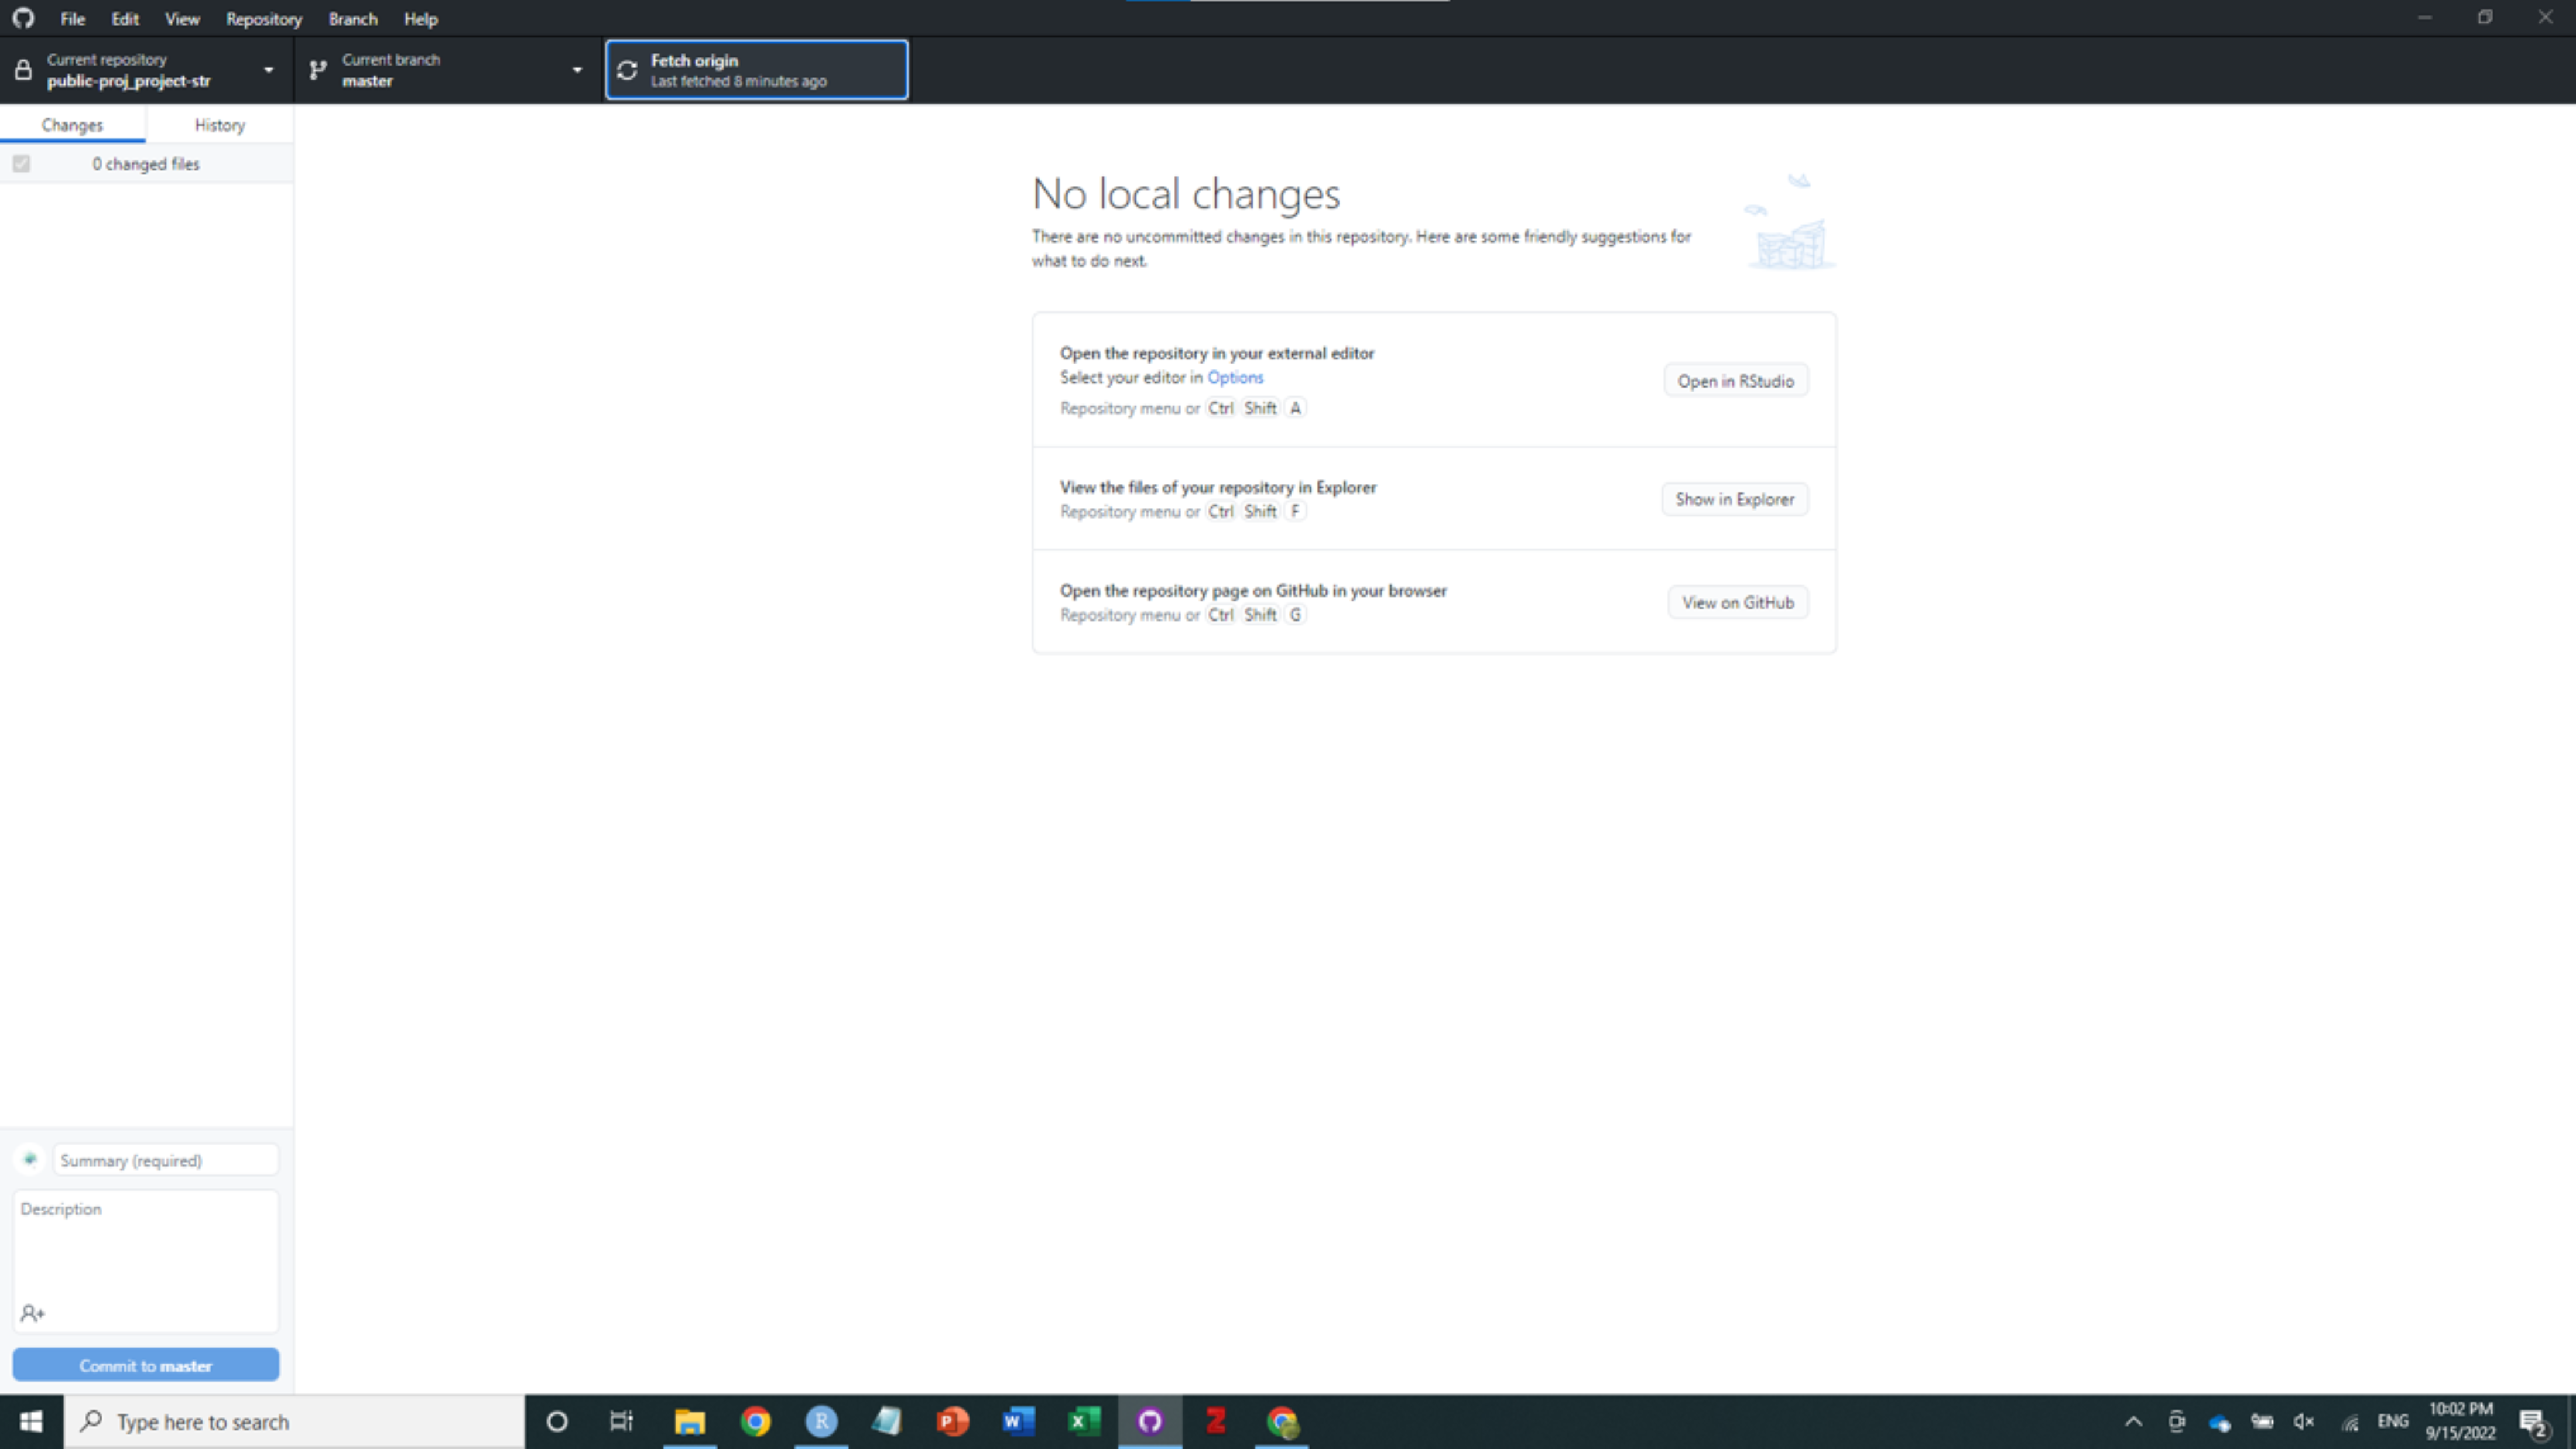
\includegraphics[width=61.11in]{image/git_image02} 

}

\caption{GUI for GitHub Desktop}\label{fig:gitdesktop1}
\end{figure}

Hit \texttt{current\ repository} (top left) and \texttt{Add} \textgreater{} \texttt{Add\ existing\ repository} (Figure \ref{fig:gitdesktop2}):

\begin{figure}

{\centering 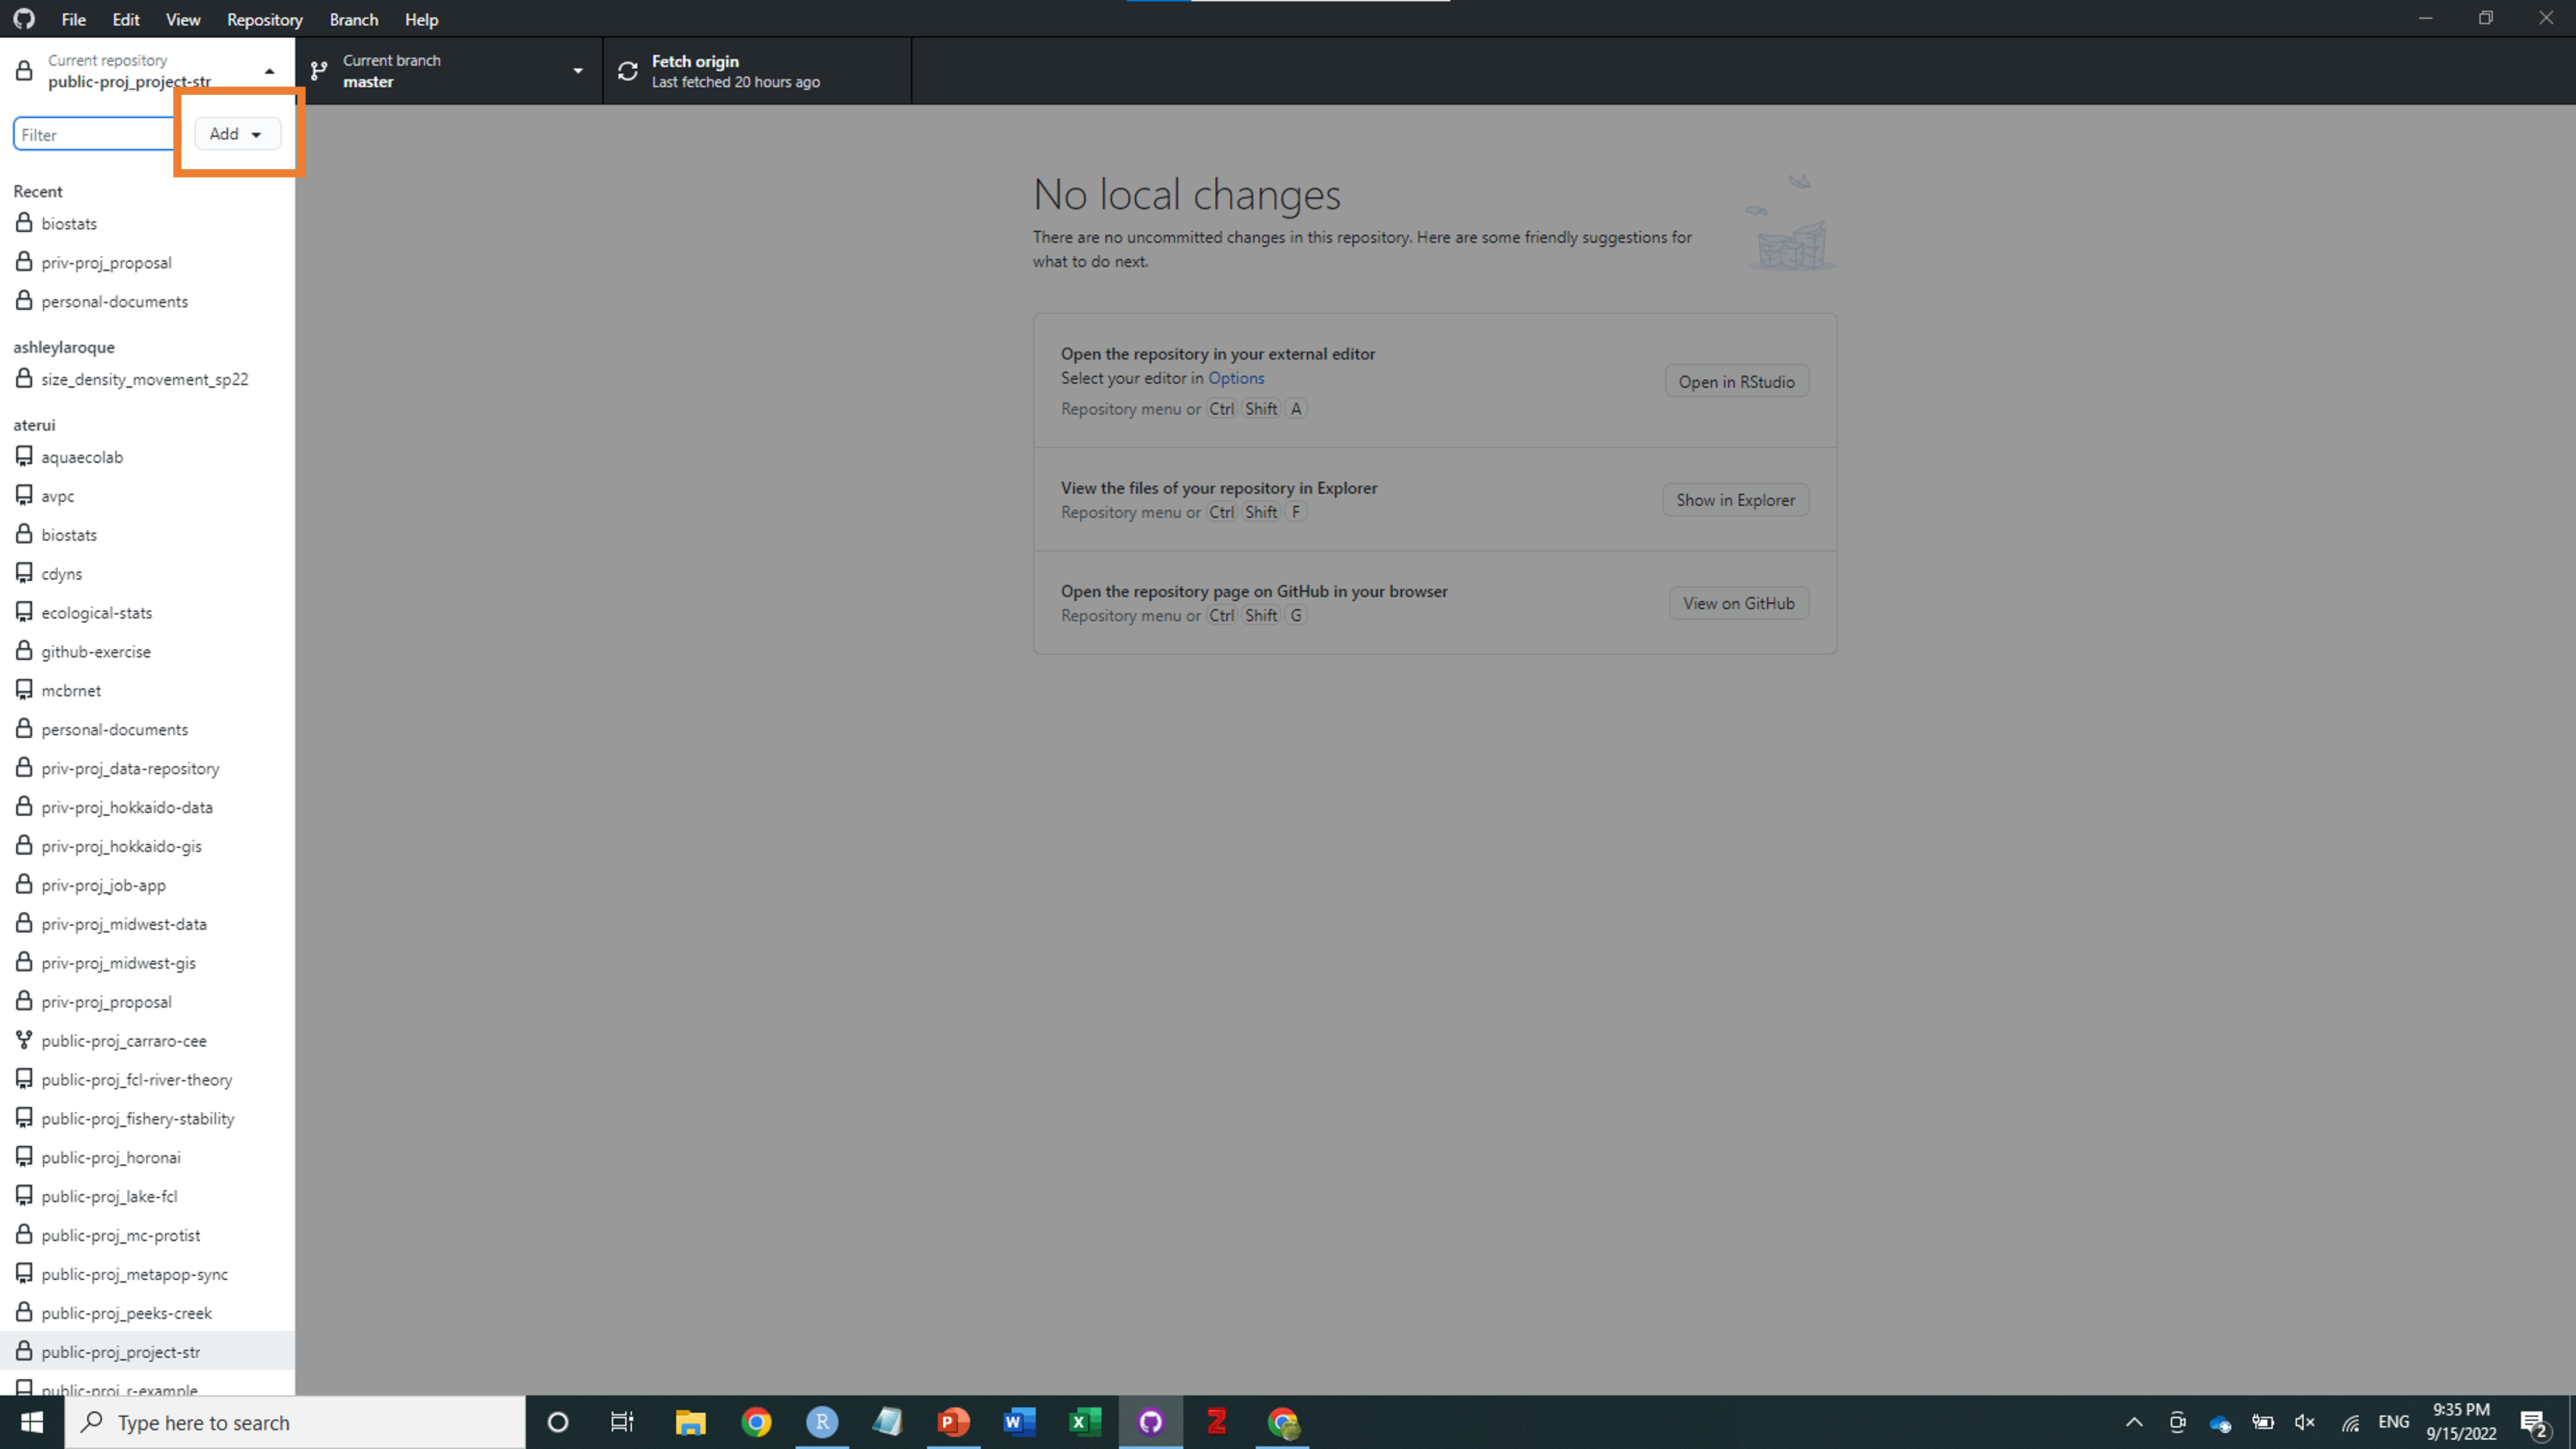
\includegraphics[width=61.11in]{image/git_image03} 

}

\caption{Add dropdown on the top left}\label{fig:gitdesktop2}
\end{figure}

\hypertarget{commit}{%
\subsection{Commit}\label{commit}}

GitHub Desktop will prompt you to enter a local path to your \emph{Git} repository. Browse and select your directory of the \texttt{R\ Project} - the local Git repository will show up in the list of repositories in \emph{GitHub Desktop} (left side bar in Figure\ref{fig:gitdesktop2})\emph{.} Now, you are ready to \textbf{Commit} your files to \emph{Git}! Commit is the procedure to record your file change history in \emph{Git}. To make this happen, click your \emph{Git} repository on GitHub Desktop, and you will see the following:

\begin{figure}

{\centering 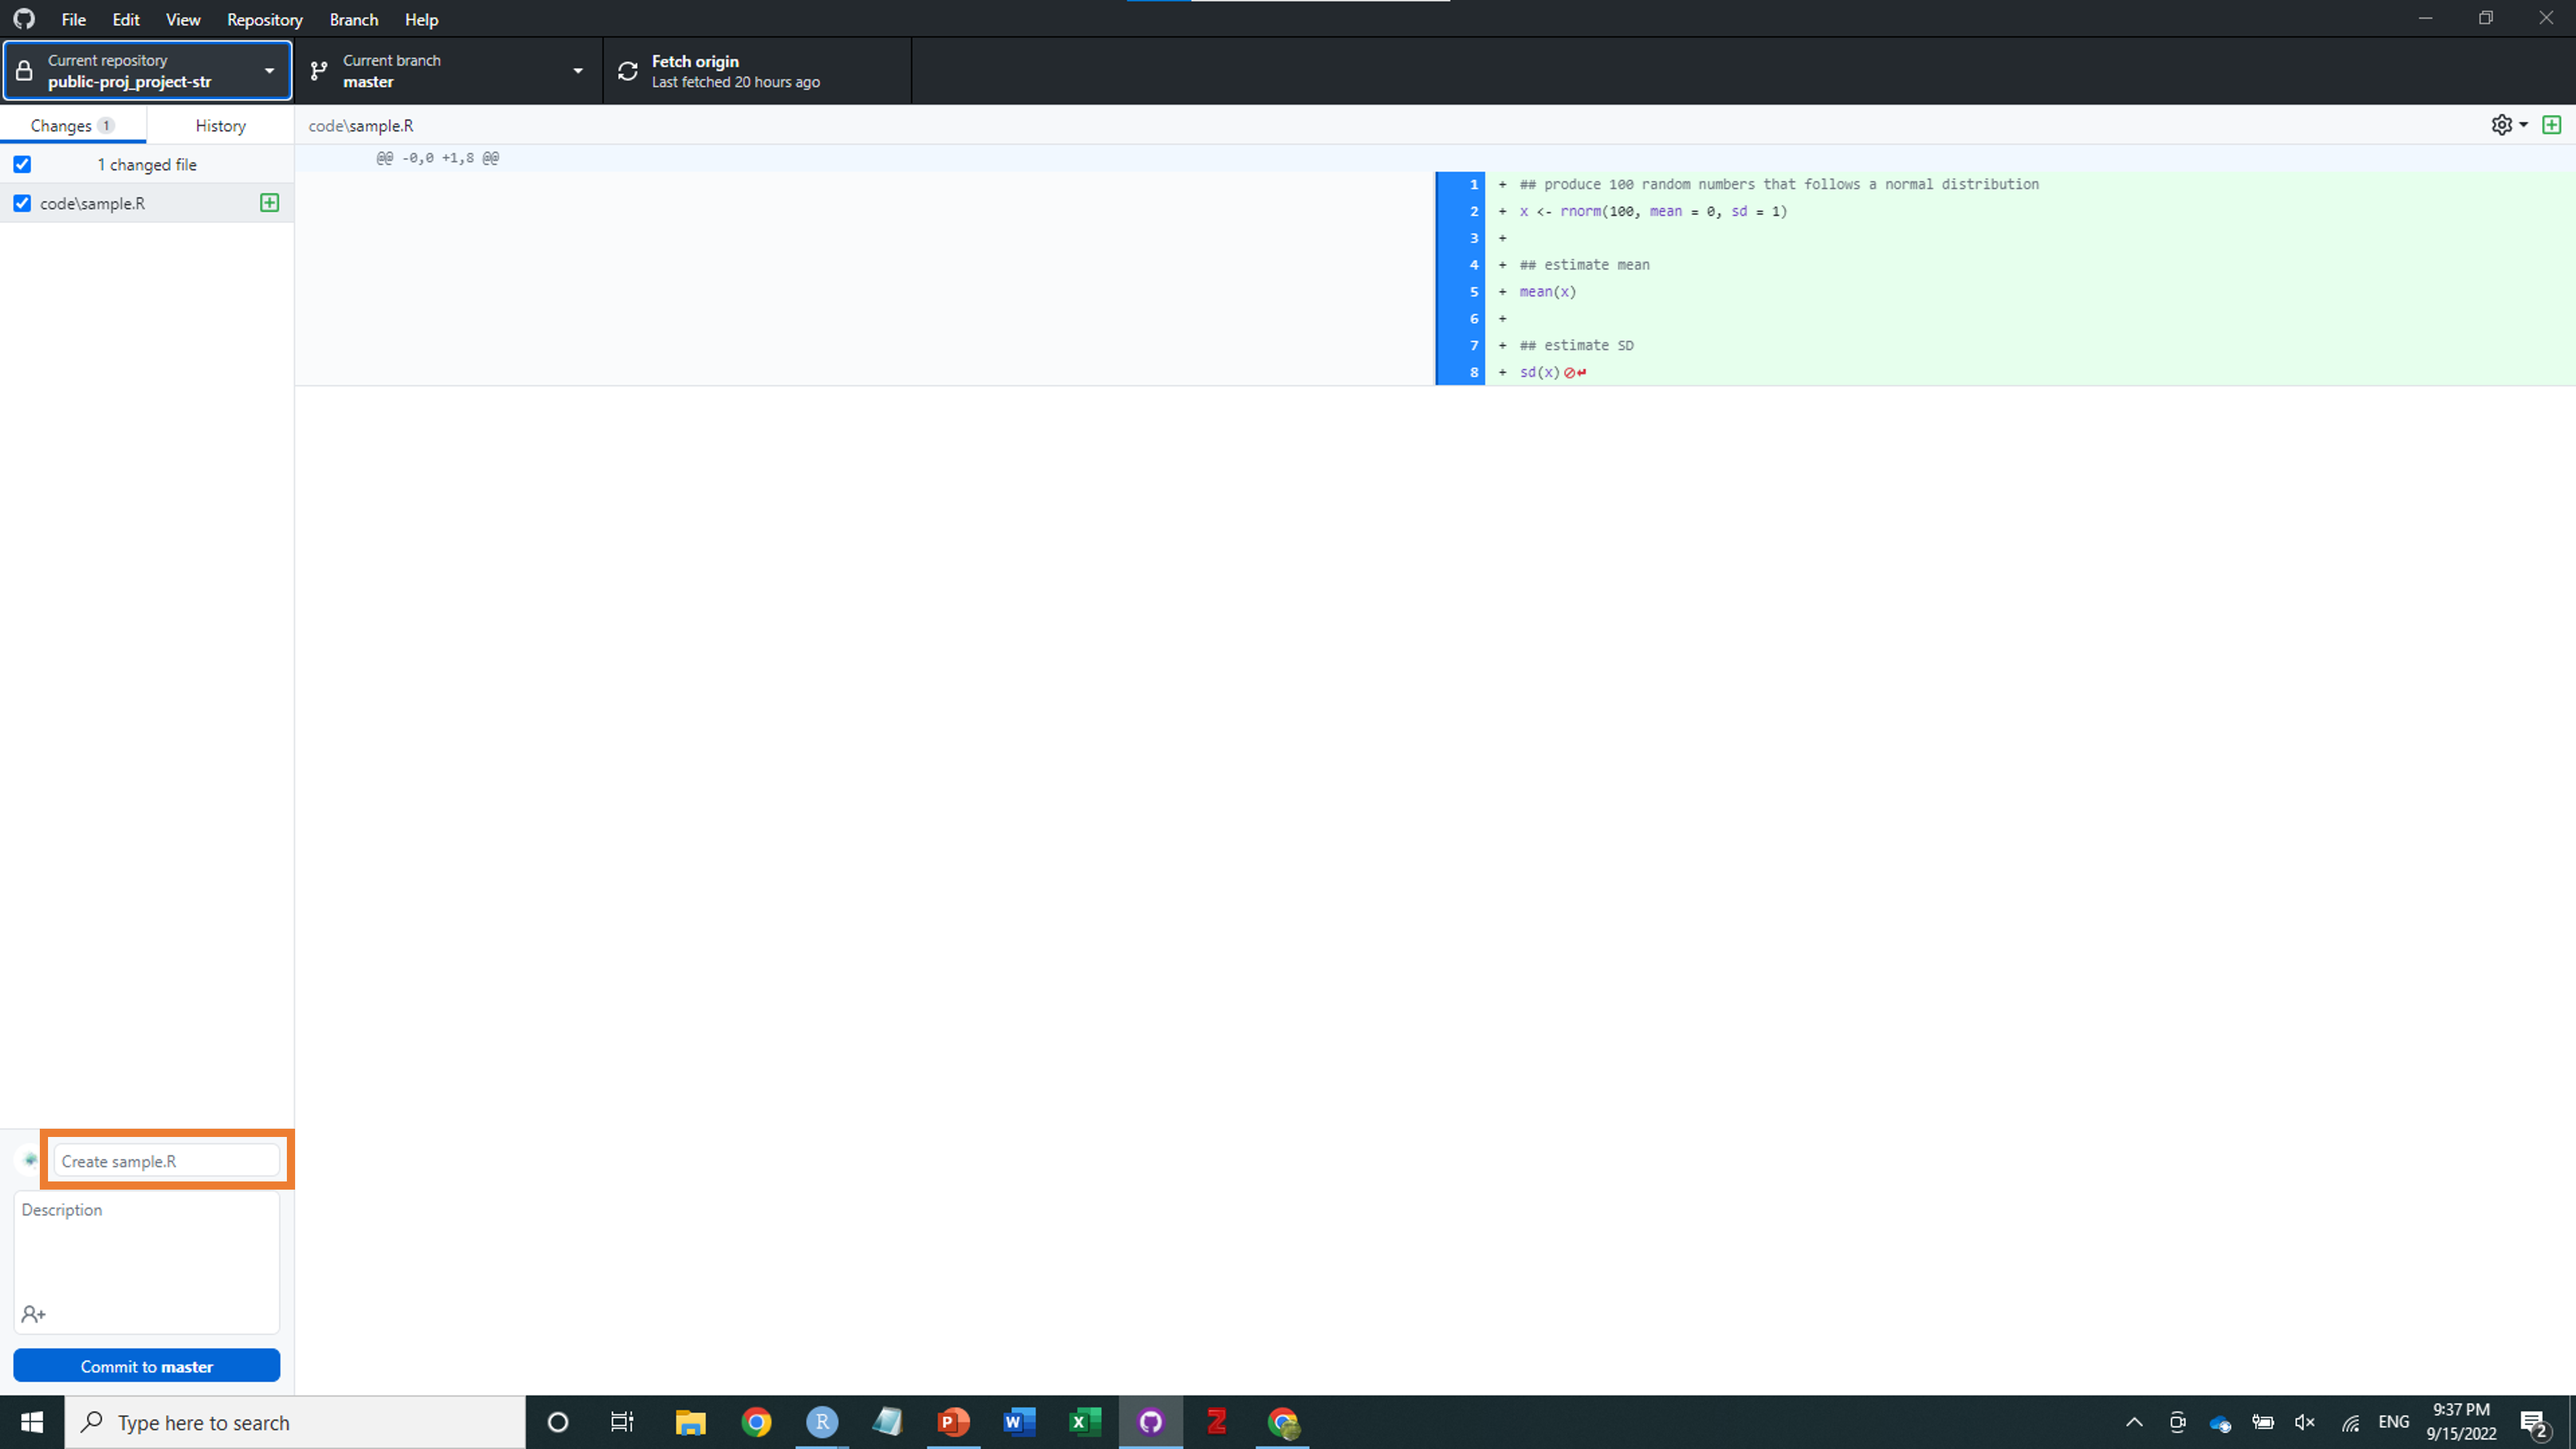
\includegraphics[width=61.11in]{image/git_image04} 

}

\caption{You will see `Create sample.R` or `summary (required)` on the bottom left}\label{fig:gitdesktop3}
\end{figure}

At this stage, your file (\texttt{.R} or else) is saved onto your local directory, \textbf{but has not been recorded in \emph{Git} as a change history.} To make a Commit, the first thing to do is to choose a file(s). There are checkboxes next to each of the new files. If this box is checked, you are going to commit changes to \emph{Git}. Once you selected the files you want to make a commit, go to the bottom left of the window. There is a small box saying \texttt{summary\ (required)} or \texttt{Create\ sample.R}.This is the place where you can put any title that describes what you did in this commit, and \textbf{you cannot Commit unless you enter this information!} For example, I would write \texttt{initial\ commit} for this exercise - from the second commit, you should put a more informative commit message so you can track changes when needed. You can google recommendations for how to write commit titles/descriptions. Then hit \texttt{commit\ to\ master}. \textbf{Now, changes to the selected files have been recorded in \emph{Git}!}

\hypertarget{push}{%
\subsection{Push}\label{push}}

Remember, your changes are recorded in your local computer \textbf{but not published in your online repository!} To send local changes to the online \emph{GitHub} repository, you will need to \textbf{Push} commits via \emph{GitHub Desktop}. Push is the procedure to send your Commit(s) to \emph{GitHub}. Once you do a Commit, \emph{GitHub Desktop} will ask you whether you want to Push it to an online repository (Figure \ref{fig:gitdesktop4}). If this is the first push, there is no corresponding repository on \emph{GitHub} tied to your local repository, so \emph{GitHub Desktop} will ask you if you want to publish it on \emph{GitHub} (NOTE: although it says `publish', your repository will remain private unless you explicitly tell \emph{Git Desktop} to make it public). If you are comfortable with the changes you made, \textbf{Push} it!

\begin{figure}

{\centering 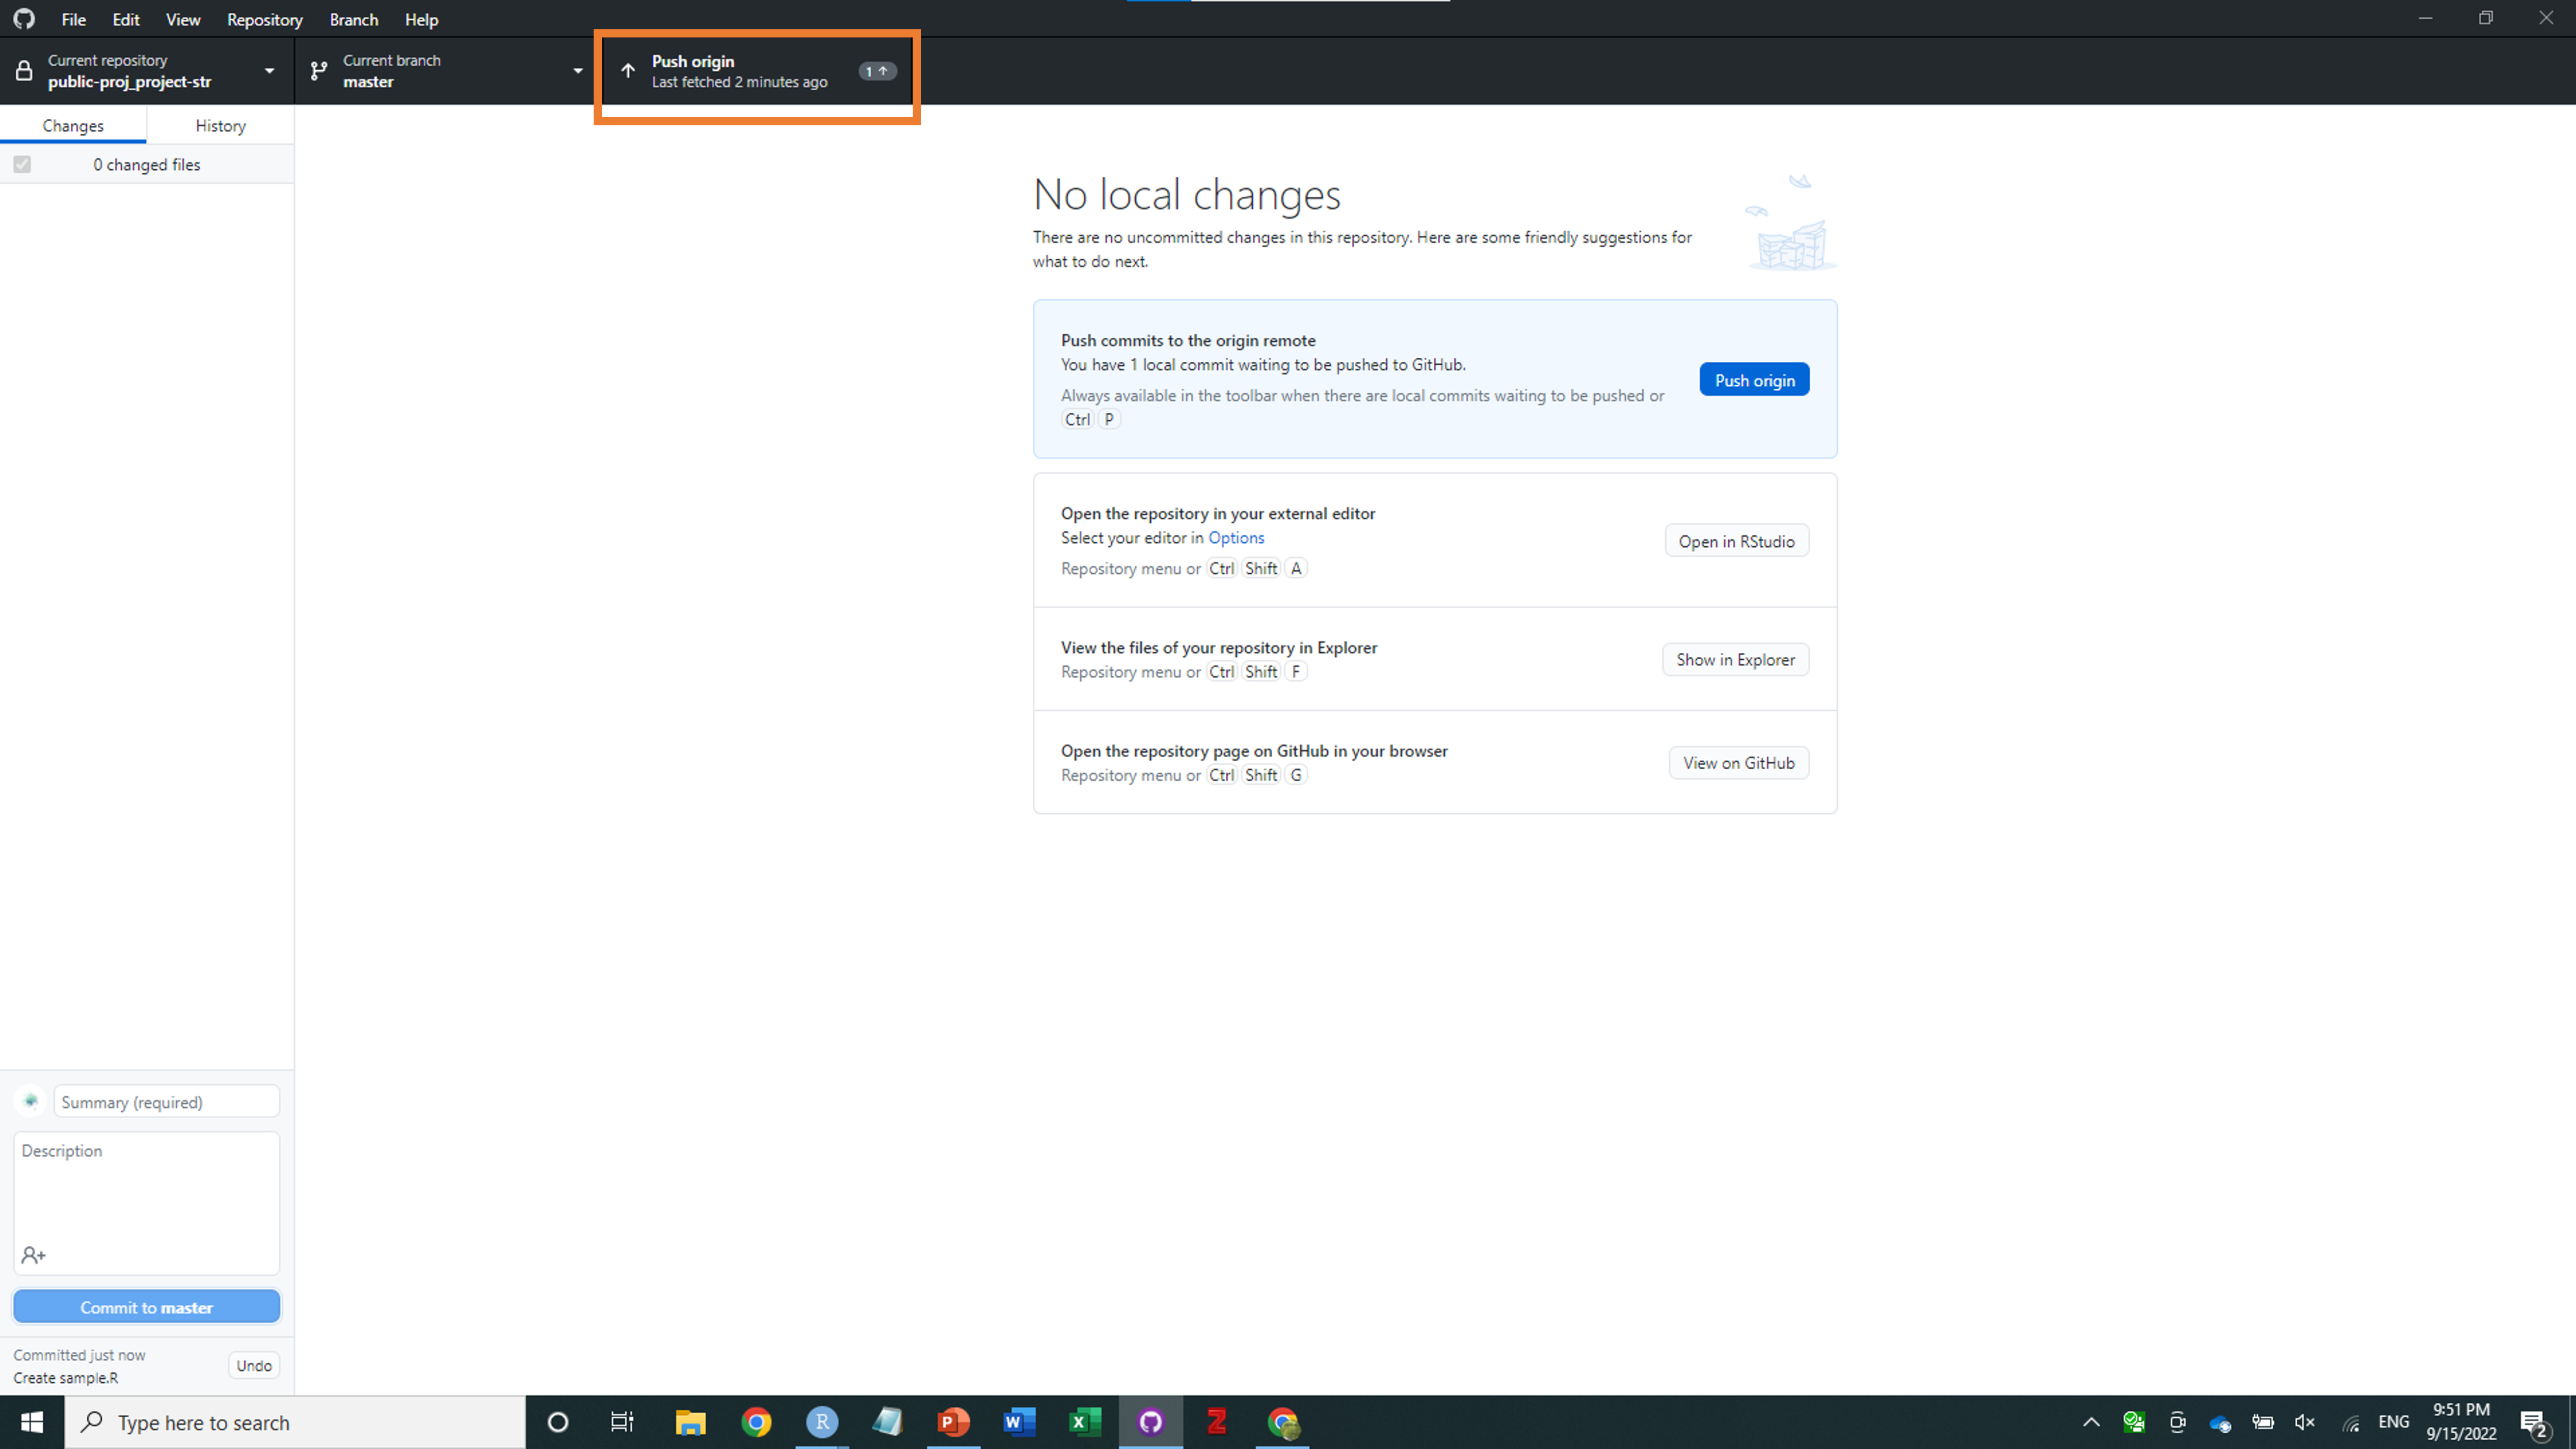
\includegraphics[width=61.11in]{image/git_image05} 

}

\caption{To Push your code, hit the highlighted menu button}\label{fig:gitdesktop4}
\end{figure}

\hypertarget{edit}{%
\subsection{Edit}\label{edit}}

We went through how we get things uploaded onto \emph{GitHub}, but what happens if we make changes to existing files? To see this, let's make a minor change to your R script. We have created a file \texttt{sample.R}:

\begin{Shaded}
\begin{Highlighting}[]
\DocumentationTok{\#\# produce 100 random numbers that follows a normal distribution}
\NormalTok{x }\OtherTok{\textless{}{-}} \FunctionTok{rnorm}\NormalTok{(}\DecValTok{100}\NormalTok{, }\AttributeTok{mean =} \DecValTok{0}\NormalTok{, }\AttributeTok{sd =} \DecValTok{1}\NormalTok{)}

\DocumentationTok{\#\# estimate mean}
\FunctionTok{mean}\NormalTok{(x)}

\DocumentationTok{\#\# estimate SD}
\FunctionTok{sd}\NormalTok{(x)}
\end{Highlighting}
\end{Shaded}

Edit this as follows:

\begin{Shaded}
\begin{Highlighting}[]
\DocumentationTok{\#\# produce 100 random numbers that follows a normal distribution}
\NormalTok{x }\OtherTok{\textless{}{-}} \FunctionTok{rnorm}\NormalTok{(}\DecValTok{100}\NormalTok{, }\AttributeTok{mean =} \DecValTok{0}\NormalTok{, }\AttributeTok{sd =} \DecValTok{1}\NormalTok{)}

\DocumentationTok{\#\# estimate mean}
\FunctionTok{median}\NormalTok{(x)}

\DocumentationTok{\#\# estimate SD}
\FunctionTok{var}\NormalTok{(x)}
\end{Highlighting}
\end{Shaded}

After making this change, go to \emph{GitHub Desktop} again. \emph{GitHub Desktop} automatically detects the difference between the new and old files and shows which part of the script has been edited! This helps coding quite a bit:

\begin{figure}

{\centering 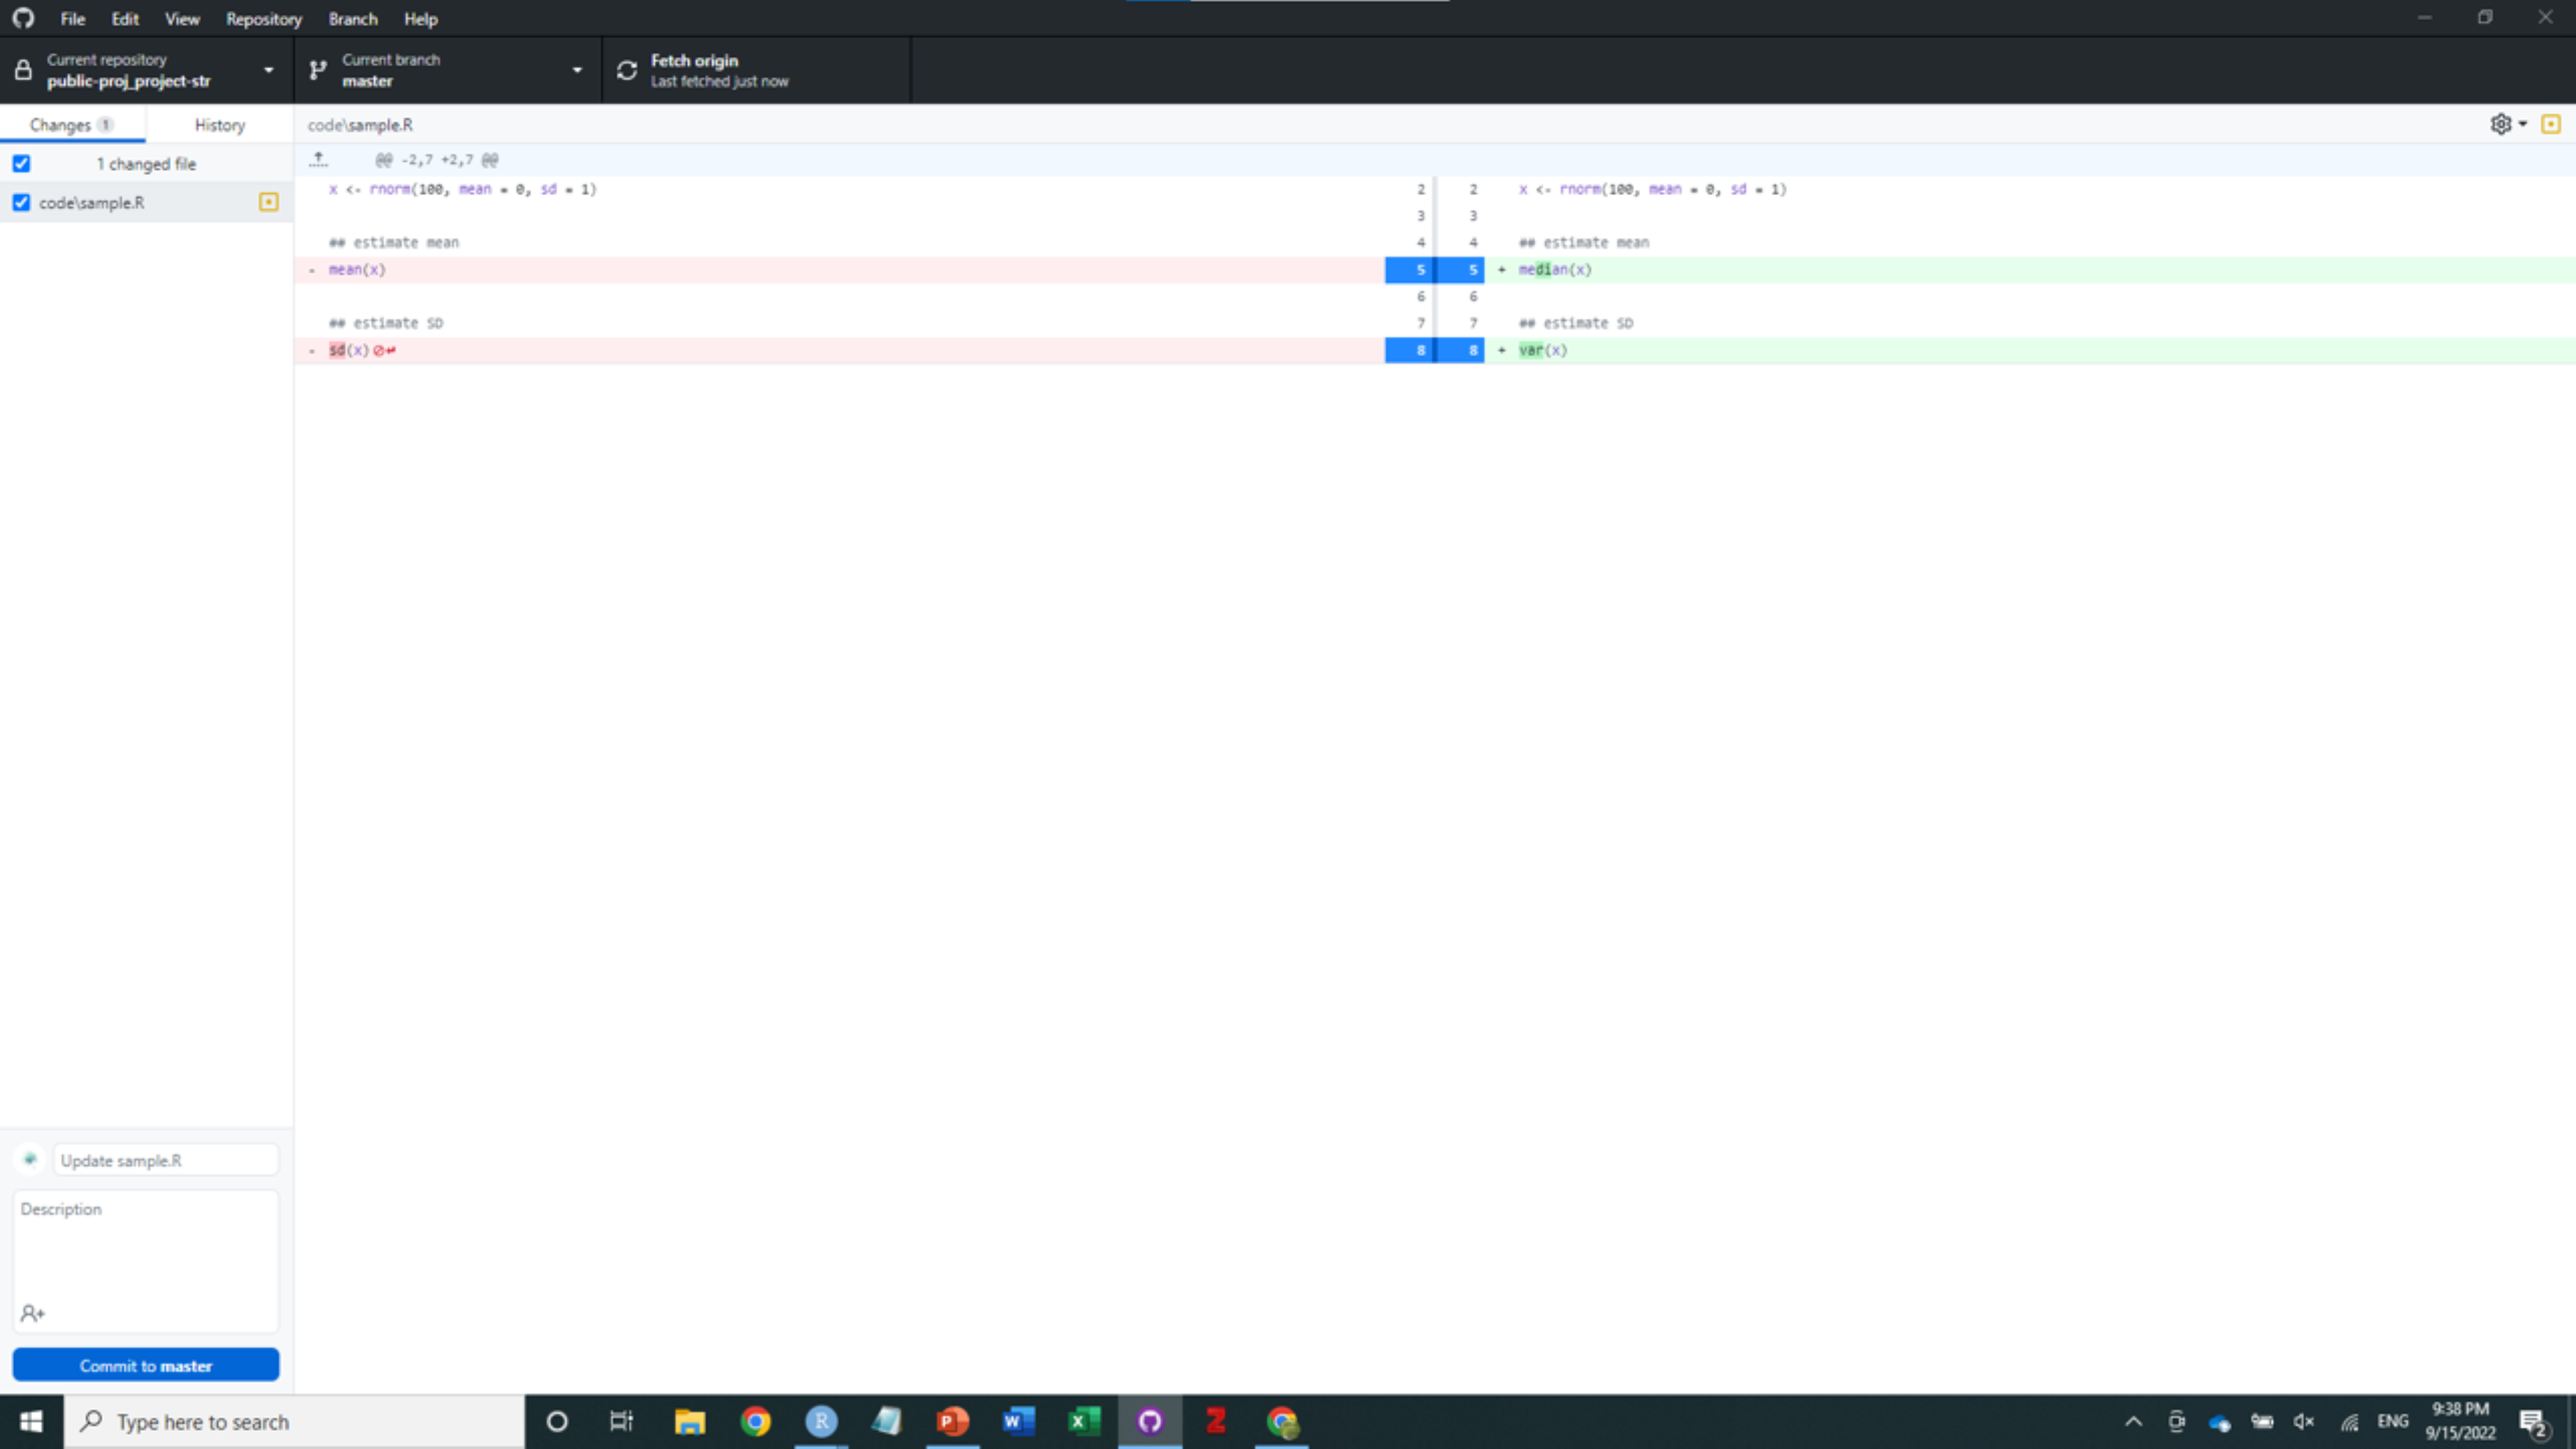
\includegraphics[width=61.11in]{image/git_image06} 

}

\caption{Git detects edits to your codes}\label{fig:gitdesktop5}
\end{figure}

\end{document}
